\documentclass[a4paper, 11pt, nofootinbib]{article}

\setcounter{tocdepth}{3}
\setcounter{secnumdepth}{3}
\usepackage{amsmath}
\usepackage{comment} % enables the use of multi-line comments (\ifx \fi) 
\usepackage{lipsum} %This package just generates Lorem Ipsum filler text. 
\usepackage{fullpage} % changes the margin
\usepackage[utf8]{inputenc}
\usepackage{gensymb}
\usepackage{graphicx}
\usepackage{booktabs}% http://ctan.org/pkg/booktabs
\usepackage{makecell}
\usepackage{tabularx}
\usepackage[table]{xcolor}
\usepackage{array}
\usepackage{wrapfig}
\usepackage{subcaption}
\usepackage{csquotes}
\usepackage{lscape}
\usepackage{afterpage}
\usepackage{geometry}
\usepackage{listings}
\usepackage{xcolor}
\usepackage{ulem}
\usepackage{chngcntr}
\usepackage{multicol}

%Tabellenheadings
\renewcommand*{\thead}[1]{\bfseries #1}

%Ermöglicht bullet-points in Tabellen
\newcommand \tabitem{\makebox[1em][r]{\textbullet~}}

%Abbildungen werden pro Kapitel nummeriert (Abb. 1.4, Abb. 4.7 etc)
\counterwithin{figure}{section}

\geometry{a4paper, margin=1in}

%Bilder haben die Unterschrift Abb. anstelle von Figure
\renewcommand{\figurename}{Fig..}

%\code{Text} formatiert Text als monospace Schrift
\newcommand{\code}[1]{\texttt{#1}}


%Wie sollen Code-Snippets mit \lstinline|code| aussehen?
\lstset{frame=tblr,
	captionpos=b,
	language=c,
	aboveskip=3mm,
	belowskip=3mm,
	showstringspaces=false,
	columns=flexible,
	basicstyle={\small\ttfamily},
	numbers=left,
	numberstyle=\tiny\color{gray},
	keywordstyle=\color{blue},
	commentstyle=\color{darkgreen},
	stringstyle=\color{violet},
	breaklines=true,
	breakatwhitespace=true,
	tabsize=3
}

%RGB-Definition von eiigen Farben
\definecolor{system}{RGB}{141,0,76}
\definecolor{inhalt}{RGB}{2,47,99}
\definecolor{darstellung}{RGB}{116,117,117}
\definecolor{nutzung}{RGB}{207,2,127}
\definecolor{darkgreen}{RGB}{39,117,1}

\begin{document}
\title{Summary Micro-Controller FS18}
\author{Alex Neher}
\maketitle

\tableofcontents
\newpage

\graphicspath{{./Pictures/}}

\section{Components}
Microcontrollers are so called \textbf{Single Chip} Computer, meaning everything is on a single PCB, as opposed to e.g. a 'normal' PC.

\begin{wrapfigure}[8]{R}{0.5\textwidth}
	\centering
	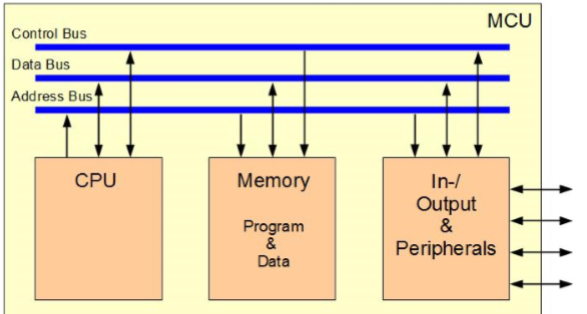
\includegraphics[keepaspectratio=true,height=10\baselineskip]{architecture.PNG}
	\caption{Von-Neumann Architecture}
	\label{fig:arch}
\end{wrapfigure}

MC consist of at least four components:

\begin{description}
	\item[CPU: ] Central Processing Unit
	\item[Memory: ] Where programs and data are stored
	\item[IO/Input-Output: ] Communication with Peripherals
	\item[Bus-System: ] Connects the components
\end{description}

\vspace{10px}

\noindent There are two different architectures:

\begin{description}
	\item[Von-Neumann: ] One shared bus for program and data. Program and data are in the same memory. Often found in low-cost MCs
	\item[Harvard: ] Two separate bus systems for program and data. Often found in high-performance MCs
\end{description}
\vspace{10px}

\noindent Usually, a read/write-operation goes through four steps:

\begin{enumerate}
	\item CPU puts the address on the address bus
	\item Either the memory or the IO claim the address as their
	\item CPU tells the component via the control bus whether the operation is read or write
	\item 
		\subitem \textit{read: } The memory or IO places the data of the requested address on the data bus
		\subitem \textit{write: } The CPU writes the data on the mentioned address via data bus
\end{enumerate}

\newpage

\section{Numerical systems}
In MC, variables and constants are seldom stored as decimal value. Rather they're either stored as a binary or a hexadecimal value. 

In general, mathematical terms an $n$-digit integer to the base $B$ can be expressed as:

\[ \scalebox{1.5}{$ \sum_{i=0}^{n-1} x_{i} * B^i = X_{0} * B^0 + x_{1} * B^2 + [...] + x_{n-1} * B^{n-1} $} \]

\noindent Or easier: \textit{Multiply the $n$-th digit of the integer with $B^{n-1}$ starting from the right} with n = 0

\subsection{Example}

\noindent $1100'0101_{2}$ (binary) to decimal \\
$
	= 1*2^0 + 0*2^1 + 1*2^2 + 0*2^3 + 0*2^4 + 0*2^5 + 1*2^6 + 1*2^7 \\
	=   1   +   0   +   4   +   0   +   0   +  0   +   64   +  128 \\
	=   \underline{\underline{197_{10}}}
$

\noindent If you have to convert a number between two 'exotic' systems, say base 8 to base 3, it's usually easier to convert it to decimal first and then convert it to the desired system again ($x_{8} \rightarrow x_{10} \rightarrow x_{3}$). An exception to that is binary to hexadecimal and vice versa. One digit in hexadecimal represents four digits in binary, so you can directly convert blocks of four:

\noindent $1100'0101_{2}$ to hexadecimal:
\vspace{10px}

\noindent
$1100 = 0*2^0 + 0* 2^1 + 1*2^2 + 1*2^3 = 0 + 0 + 4 + 8 = 12_{10} = C_{16} \\
0101 = 1 * 2^0 + 0*2^1  + 1*2^2 + 0*2^3 = 1 + 0 + 4 + 0 = 5_{10} = 5_{16} \\
\rightarrow 1100'0101_{2} = C5_{16}
$

\subsection{Two's Complement}
Especially in MC-technology, signed numbers (that can also be negative) are mostly stored as \textit{two's complement}. You basically take the binary number, invert every digit and add one. So -28 would be stored as
\vspace{10px}

\noindent
$ 28_{10} = 16 + 8 + 4 = 2^2 + 2^3 + 2^4 = 0001'1100_{2}$ \\
invert \\
$ 0001'1100 \rightarrow 1110'0011$\\
add one \\
$1110'0011 + 1 = \underline{\underline{1110'0100}}$

\newpage

\section{Logic Gates}
\begin{figure}[htb]
	\centering
	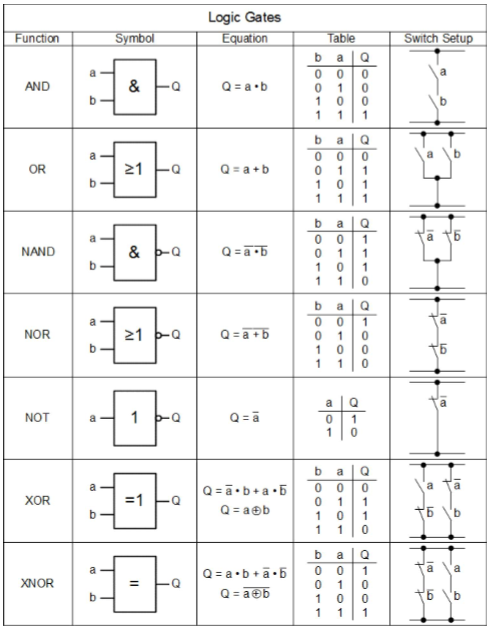
\includegraphics[keepaspectratio=true,height=22\baselineskip]{logicGates.PNG}
	\caption{Fundamental logic-Gates used in MCs}
	\label{fig:logicGates}
\end{figure}

\begin{figure}[htb]
	\centering
	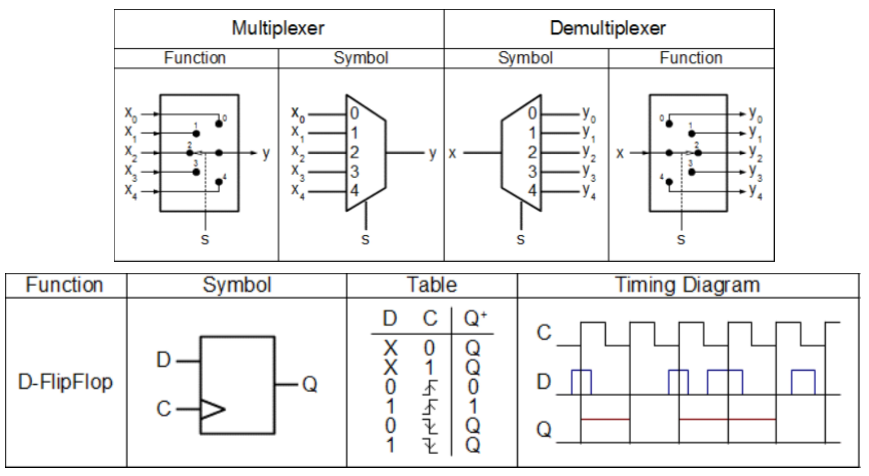
\includegraphics[keepaspectratio=true,height=12\baselineskip]{flipflop.PNG}
	\caption{Visualisation of the (de)multiplexer and the flipflop}
	\label{fig:multFlip}
\end{figure}

\begin{description}
	\item[Multiplexer: ] The multiplexer is a combinational logic circuit, which allows us to select one of many input lines and route it to the single, common output line. The demultiplier does the exact opposite: it takes one input and you can select to which output line it is routed
	\item[FlipFlop: ] Idunno %TODO: Get WTF FlipFlops are
\end{description}

\newpage

\section{Instruction Set Cycle}

\begin{wrapfigure}[8]{L}{0.5\textwidth}
	\centering
	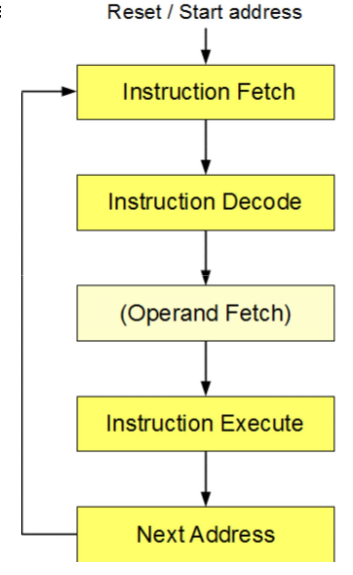
\includegraphics[keepaspectratio=true,height=20\baselineskip]{instructionCycle.PNG}
	\caption{Visualisation of the Instruction Set Cycle}
	\label{fig:instCycle}
\end{wrapfigure}

The way a CPU executes instructions can be shortened to \textbf{FDE}. It stands for \textbf{F}etch, \textbf{D}ecode \textbf{E}xecute. 
\vspace{10px}
S
\noindent As can be seen in fig. \ref{fig:instCycle}, the CPU first fetches the instruction from the memory, then it decodes it and decides if it has to fetch a second operand (e.g. for an addition). Afterwards it executes said instruction and moves on to the next address.

\vspace{200px}

\section{Assembler}
\subsection{Directives}
Put simply, Assembler directives are instructions that direct the assembler to do something:
\begin{center}
\begin{tabular}{|p{2cm}|p{5cm}|p{4cm}|p{5cm}|}
	\hline
	\thead{Directive} & \thead{Description} & \thead{Example} & \thead{Explanation} \\
	\hline
	SECTION & Defines the beginning of a relocatable section & ConstSec: SECTION & Puts the whole ConstSec-Section in the same RAM-section\\
	\hline
	EQU & Assign an expression to a name. Not redefinable & MaxElement: EQU 20 & search-and-replace every \textit{MaxElement} in the code with 20\\
	\hline
	DC & Defines one or more constants and theirnames & DC B \$AA & Pointer to address \$AA at every \textit{Alarm}\\
	\hline
	DS & Allocates memory to variables & DS W 3 & Reserves 3 words of RAM. 1 Word = 2 Bytes\\
	\hline
\end{tabular}
\end{center}

\newpage

\subsection{Addressing modes}
There are six different addressing modes that are supported by our CPU:

\begin{description}
	\item[Immediate: ] 1 Byte operand in the instruction \\
		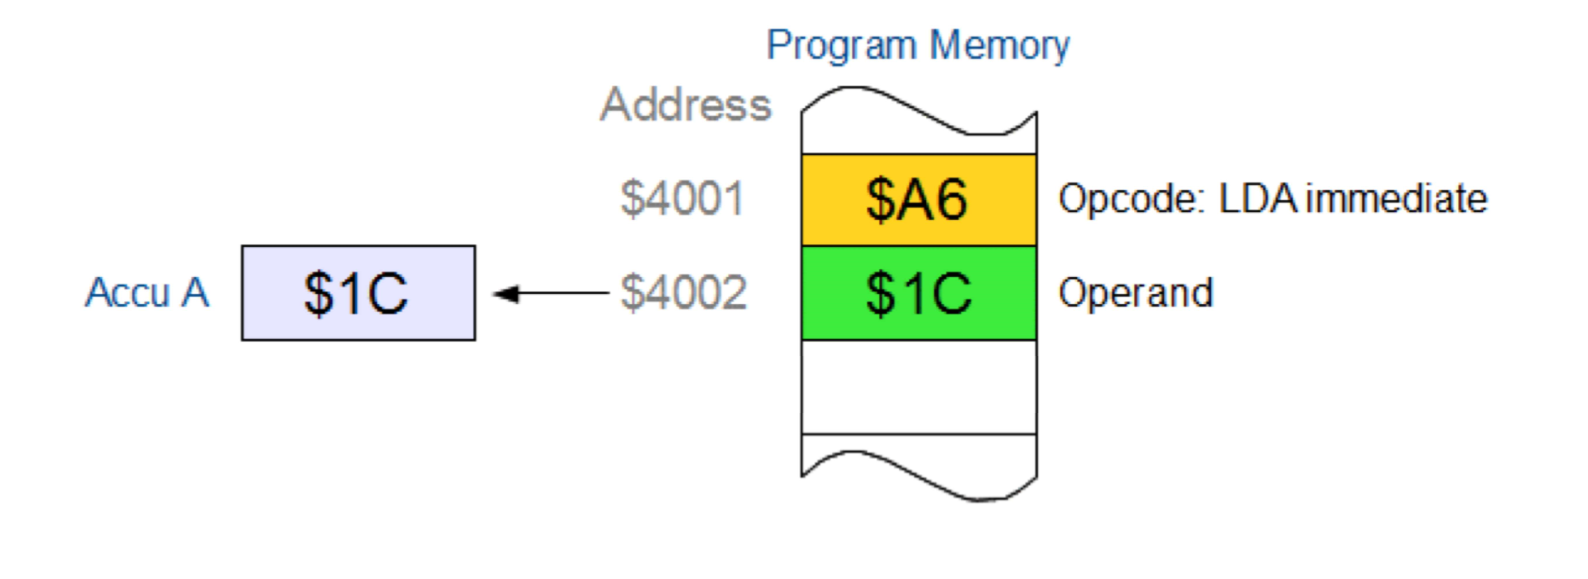
\includegraphics[keepaspectratio=true, height=10\baselineskip]{immAdd.PNG}
	\item[Inherent: ] No operand required \\
		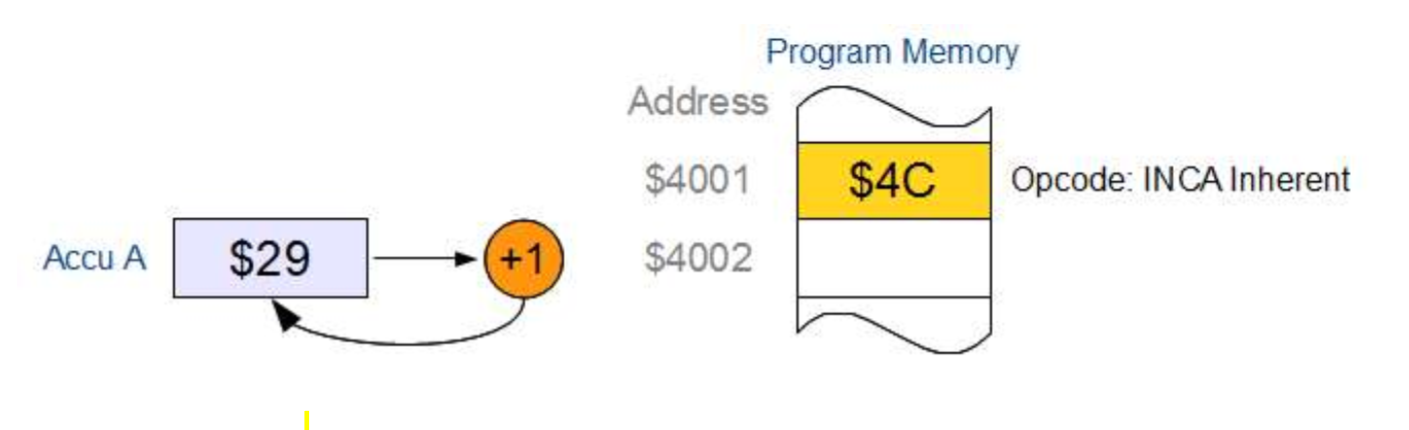
\includegraphics[keepaspectratio=true, height=10\baselineskip]{inhAdd.PNG}
	\item[Direct: ] Operands must be stored in the Direct Page (From \code{0x0000} to \code{0x00AF}) \\
		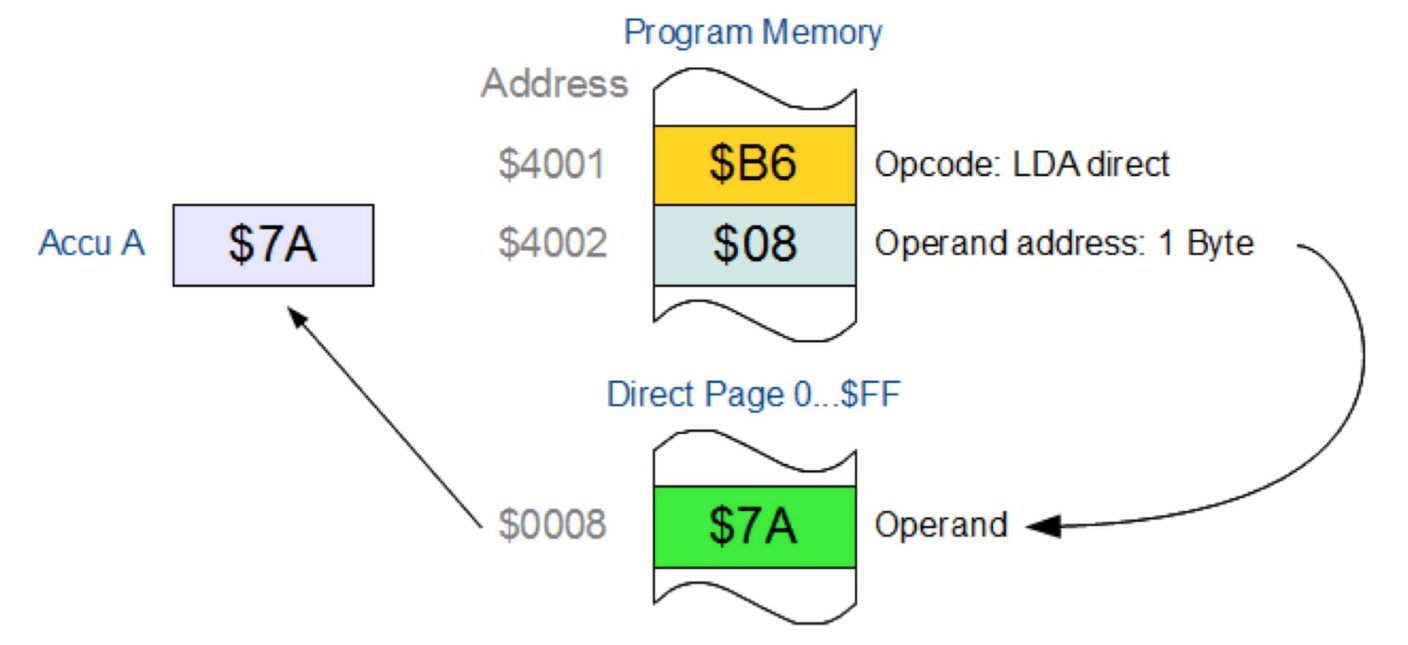
\includegraphics[keepaspectratio=true, height=10\baselineskip]{dirAdd.PNG}
	\item[Extended: ] Operand can be stored in the whole 64k Memory \\	
		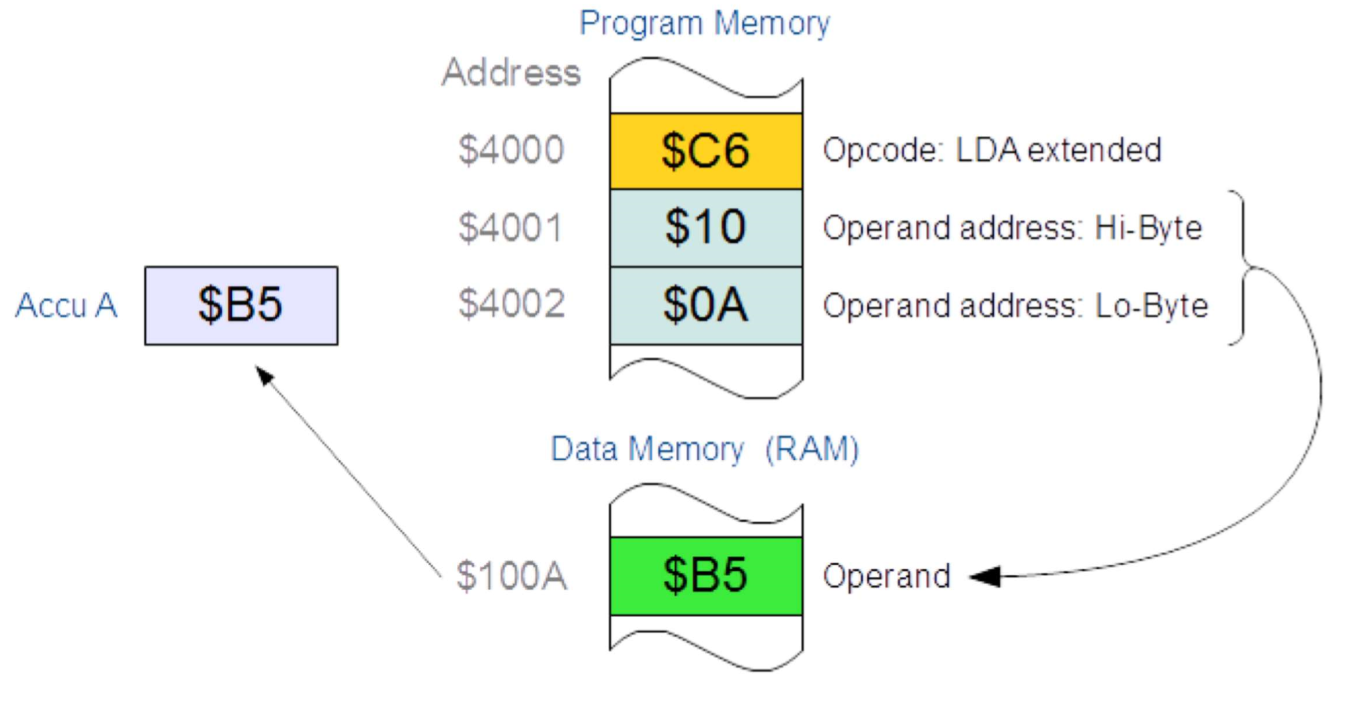
\includegraphics[keepaspectratio=true, height=10\baselineskip]{extAdd.PNG}
	\item[Indexed: ] Operand is stored in Stack Pointer or H:X Register \\
		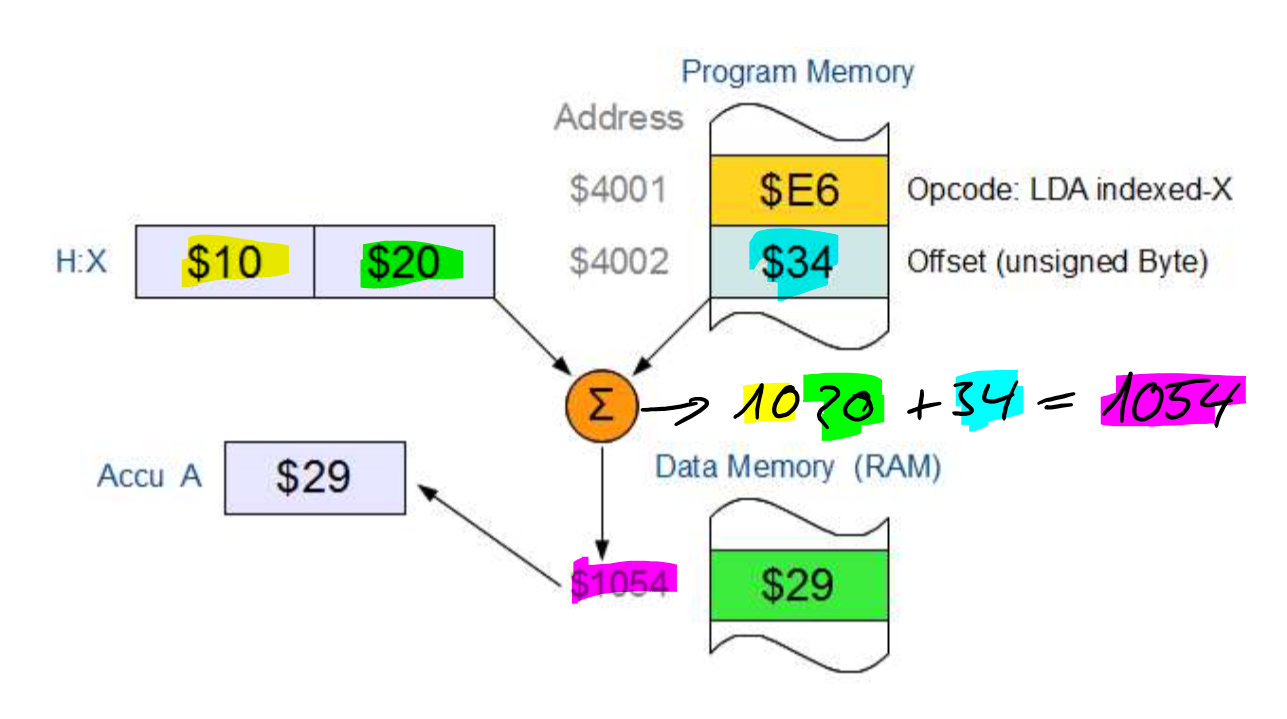
\includegraphics[keepaspectratio=true, height=10\baselineskip]{indAdd.PNG}
	\item[Relative: ] Only used with \code{BRANCH}-Instructions. Depending on outcome of the Branch \\
		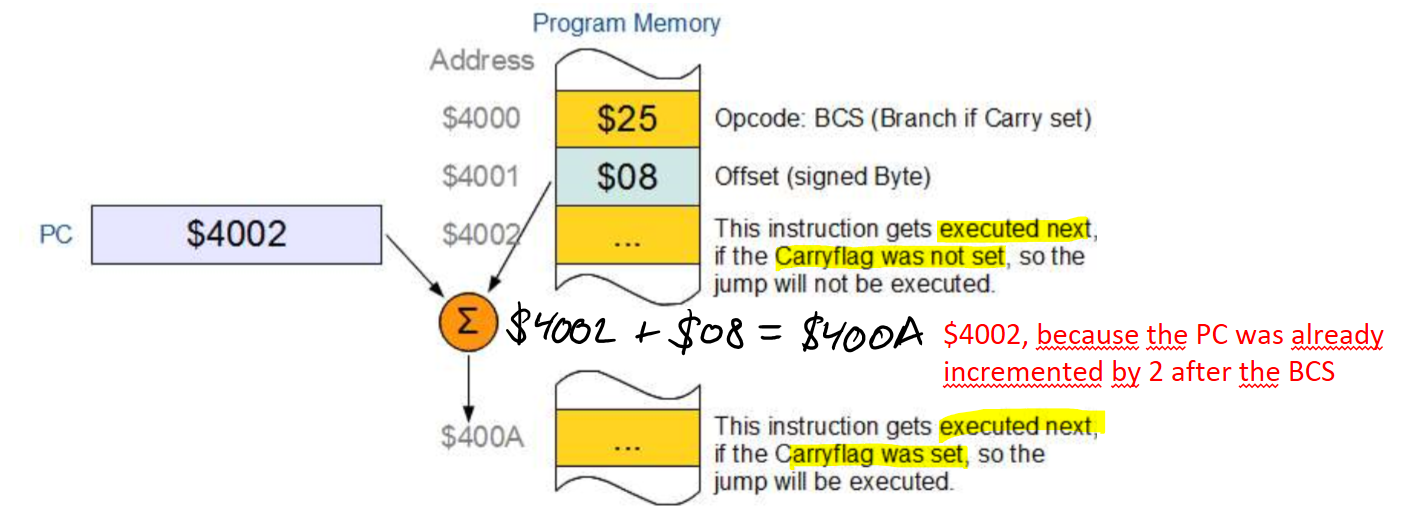
\includegraphics[keepaspectratio=true, height=10\baselineskip]{relAdd.PNG}
\end{description}

\subsection{Assembler Programming Operations}
There are three main assembler instruction types:

\begin{itemize}
	\item Data Transport
		\subitem Load
		\subitem Store
		\subitem Transfer
		\subitem Move
	\item Operations
		\subitem Arithmetic
		\subitem Logic
		\subitem Bit-Manipulation/Masking
		\subitem Shift and Rotation
	\item Branching
\end{itemize}

\subsubsection{Data Transport}
Data Transport instructions are again divided into four subtypes

\begin{figure}[htb!]
	\centering
	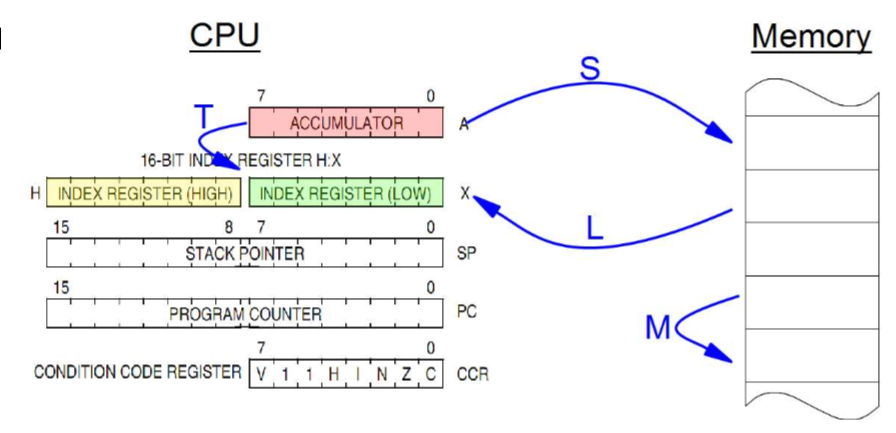
\includegraphics[keepaspectratio=true,height=15\baselineskip]{assOperations.PNG}
	\caption{Visualisation of the different data tranfers}
	\label{label}
\end{figure}

\begin{description}
	\item[Load: ] Data is moved from the memory to the CPU-Register \\
		Examples: \code{LDA, LDX, LDHX, (PULA, PULX} Stack-operations)
	\item[Store: ] Data is moved from the CPU-Register to the memory \\
		Examples: \code{STA, STX, STHX, (PSHA, PSHA} Stack-operations) 
	\item[Transfer: ] Very fast Data Transfer between CPU registers
		Examples: \code{TAP, TPA, TAX, TSX}
	\item[Move: ] Data is moved within the memory
\end{description}

\subsubsection{Arithmetic Operations}
Arithmetic operations cover the four basic mathematical operations:

\begin{description}
	\item[Addition: ] \code{ADD, ADC} (Addition with Carry Bit $\rightarrow$ supports numbers $>$ 8bit)
	\item[Subtraction: ] \code{SUB, SBC} (Addition with Carry Bit $\rightarrow$ supports numbers $>$ 8bit)
	\item[Multiplication: ] \code{MUL} Only works with unsigned numbers. Multiplies the content of the accumulator with the content of the X-register and stores the 16bit result in the X:A-registers (LSB in A, MSB in X)
	\item[Division: ] \code{DIV} Only works with unsigned numbers. Divides whatever is in the H:A-register through whatever is in the X-register. The 8bit result is stored in the accumulator. In case of an overflow or division by 0, the carry bit will be set.
\end{description}

\subsubsection{Logic and Bitmasking Operations}
Bitwise Operations change but a single bit of the operand. This can be especially useful e.g. to turn on or off LEDs, which are controlled by a register of 8 bits

\begin{description}
	\item[\code{ORA\#(B6|B3)}] \mbox{} \\
	Logical \code{OR} Operation on Bit 6 and Bit 3 $\rightarrow$ Sets \textbf{only} Bit 6 and Bit 3 in the Accumulator
	\item[\code{AND\#(B6|B3)}]\mbox{}\\
	Logical \code{AND} Operation on Bit 6 and Bit 3 $\rightarrow$ Deletes all Bits \textbf{except} Bit 6 and Bit 3
	\item[\code{BCLR n,Addr}] \mbox{}\\
	Deletes Bit n on a specific memory address
	\item[\code{BSET n, Addr}]\mbox{}\\
	Sets Bit n on a specific memory address
	\item[\code{BIT Addr}] \mbox{}\\
	\code{AND} Operation of the accumulator with the content of the address, \textit{without changing the content of either of them}
	\item[\code{CLC}] \mbox{}\\
	Clears Carry-Flag
	\item[\code{SEC}] \mbox{}\\
	Sets Carry-Flag
	\item[\code{CLI}] \mbox{}\\
	Delete Interrupt-Mask Bit ($\rightarrow$ Interrupt \textbf{enable})
	\item[\code{SEI}] \mbox{}\\
	Sets Interrupt-Mask Bit ($\rightarrow$ Interrupt \textbf{disable})
\end{description}

\subsubsection{Shift- and Rotation Operations}

\begin{figure*}[htb]
	\centering
	\begin{subfigure}[b]{0.5\textwidth}
		\centering
		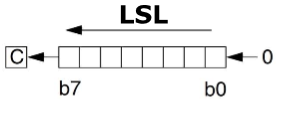
\includegraphics[keepaspectratio=true, height=5\baselineskip]{LSL.PNG}
		\caption{Logical Left-Shift}
	\end{subfigure}%
	~ 
	\begin{subfigure}[b]{0.5\textwidth}
		\centering
		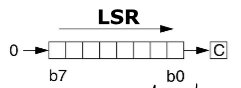
\includegraphics[keepaspectratio=true, height=5\baselineskip]{LSR.PNG}
		\caption{Logical Right-Shift}
	\end{subfigure}
	\vskip\baselineskip
	\begin{subfigure}[b]{0.5\textwidth}
		\centering
		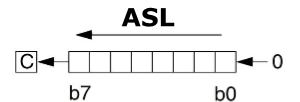
\includegraphics[keepaspectratio=true, height=5\baselineskip]{ASL.PNG}
		\caption{Arithmetic Left Shift}
	\end{subfigure}%
	~ 
	\begin{subfigure}[b]{0.5\textwidth}
		\centering
		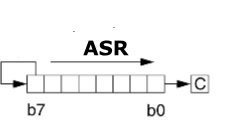
\includegraphics[keepaspectratio=true, height=7.5\baselineskip]{ASR.PNG}
		\caption{Arithmetic Right-Shift}
	\end{subfigure}
		\vskip\baselineskip
	\begin{subfigure}[b]{0.5\textwidth}
		\centering
		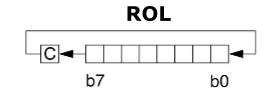
\includegraphics[keepaspectratio=true, height=5\baselineskip]{ROL.PNG}
		\caption{Rotate Left}
	\end{subfigure}%
	~ 
	\begin{subfigure}[b]{0.5\textwidth}
		\centering
		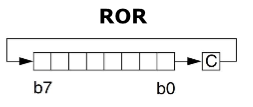
\includegraphics[keepaspectratio=true, height=7.5\baselineskip]{ROR.PNG}
		\caption{Rotate Right}
	\end{subfigure}
\end{figure*}

\noindent The Left-Shifts are an equivalent to a multiplication by two and Right-Shifts are the equivalent of a division by two:

\noindent 
$
0011'0110_{2} = 54_{10} \rightarrow LSL \rightarrow 0110'1100_{2} = 108_{10} \\
0011'0110_{2} = 54_{10} \rightarrow LSR \rightarrow 0001'1011_{2} = 27_{10}
$

\subsubsection{Branching}

\begin{tabular}{|c|c|l|}
	\hline
	\thead{Oper.}& \thead{Test} & \thead{Meaning}\\
	\hline
	\code{BEQ} & Z = 1 & Branch if equal\\
	\code{BNE} & Z = 0& Branch if not equal\\
	\hline
	\code{BCS} & C = 1& Branch if Carry\\
	\code{BCC} & C = 0& Branch if no Carry\\
	\hline
	\code{BMI} & N = 1& Branch if Negative\\
	\code{BPL} & N = 0& Branch if not Negative\\
	\hline
	\code{BGT} &$>$ & Branch if bigger (signed)\\
	\code{GHI} & &  Branch if bigger (unsigned)\\
	\hline
	\code{BGE} &$\geq$& Branch if bigger/equal (signed)\\
	\code{BHS/BCC} & & Branch if bigger/equal (unsigned)\\
	\hline
	\code{BLE} &$\leq$& Branch if lesser/equal (signed)\\
	\code{BLS} & & Branch if lesser/equal (unsigned)\\
	\hline
	\code{BLT} &$<$& Branch if lesser (signed)\\
	\code{BLO/BLS} & & Branch if lesser (unsigned)\\
	\hline
	\code{BEQ} &$=$& Branch if equal\\
	\hline
	\code{BRA} & & Branch always (Overriding SP and PC) \\
	\code{BRN} & & Branch never (Mainly used for debugging, just waits) \\
	\code{BSR} & & Brnch to subroutine (Saves SP and PC to return to main-routine) \\
	\hline
\end{tabular}
\vspace{10px}

\noindent These Branches depend on a single Bit of a memory address in the \textbf{direct pages}(\code{0x00 - 0xFF})
\begin{tabular}{|c|l|}
	\hline
	\thead{Oper.} & \thead{Meaning} \\
	\hline
	\code{BRCLR n, Addr, Label} & Branch to Label if Bit n at Address Addr is not set \\
	\hline
	\code{BRSET n, Addr, Label} & Branch to Label if Bit n at Address Addr is set \\
	\hline
\end{tabular}

\subsubsection{Comparing}
Comparing operations compare two values (kinda obvious innit?) and set the flags accordingly, but don't change the compared values:
\vspace{10px}

\noindent
\begin{tabular}{|c|l|}
	\hline
	\thead{Oper.} & \thead{Meaning} \\
	\hline
	\code{CMP opr8} & Compares content of accumulator with the 8-bit operand \\
	\hline
	\code{CPX opr8} & Compare content of X-register with 8-bit operand \\
	\hline
	\code{CPHX opr16} & Compare content of HX-register with 16-bit operand\\
	\hline
\end{tabular}

\paragraph{Example}\mbox{}\\
\begin{lstlisting}[caption={Test if a value is bigger or smaller and branch accordingly}]
LDA Op1		//Load Op1 into accumulator
CMP Op2		//Compare it to Op2 and sets Zero/Carry/Negative Flag accordingly
BMI Label	//Branch to Label if Negative flag is set (--> Op1 < Op2)
\end{lstlisting}

\newpage

\newgeometry{margin=0.5in}

\subsubsection{Flags}

\begin{figure}[htb]
	\centering
	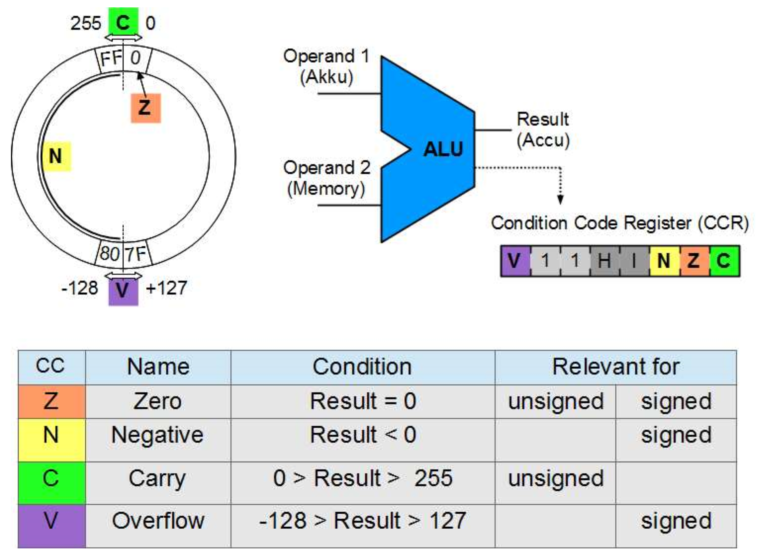
\includegraphics[keepaspectratio=true,height=19\baselineskip]{flags.PNG}
	\caption{Visualization of all supported flags}
	\label{fig:flags}
\end{figure}

\begin{figure}[htb]
	\centering
	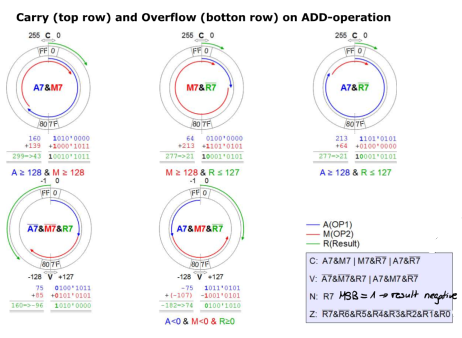
\includegraphics[keepaspectratio=true,height=19\baselineskip]{flags_add.PNG}
	\caption{Visualization of carry- and overflow-flags on Additions}
	\label{fig:flags_add}
\end{figure}

\restoregeometry
\newpage

\begin{figure}[htb]
	\centering
	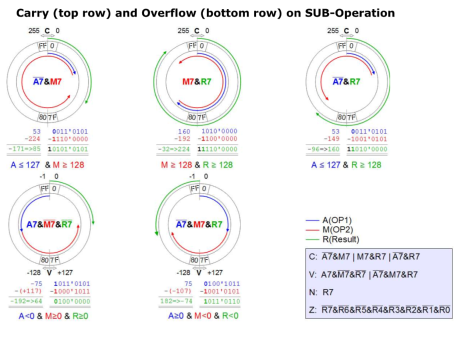
\includegraphics[keepaspectratio=true,height=20\baselineskip]{flags_sub.PNG}
	\caption{Visualization of carry- and overflow-flags on Subtractions}
	\label{fig:flags_sub}
\end{figure}

\section{Stack}
\begin{wrapfigure}[16]{R}{0.6\textwidth}
	\centering
	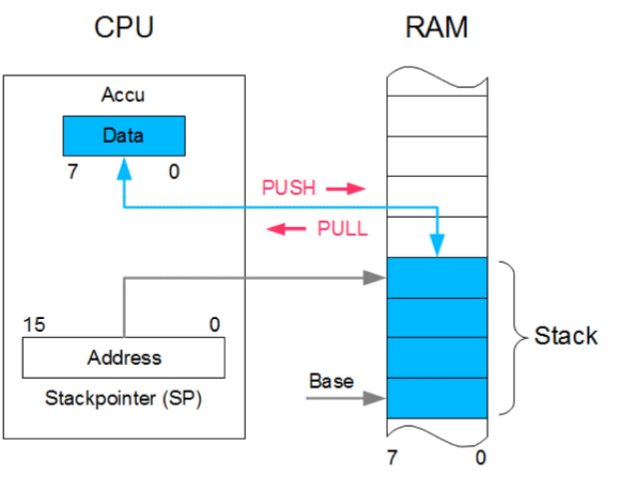
\includegraphics[keepaspectratio=true,height=18\baselineskip]{stack.PNG}
	\caption{Stack}
	\label{fig:stack}
\end{wrapfigure}

The stack is a so-called LIFO-memory (\textbf{L}ast \textbf{I}n \textbf{F}irst \textbf{O}ut), meaning whatever data is chucked on the stack last, has to be removed, before the data underneath it can be accessed.
\vspace{10px}

\noindent The Stackpointer (SP) is a pointer that always points at the next free memory place on the stack. As soon as something is pushed onto the stack (and the address the SP pointed to is therefore no longer free), it gets updated automatically. Same goes after a pull. The addresses are counted from the top of the stack, therefore the higher the stack gets, the lower the addresses.

\newpage

\begin{lstlisting}[caption={Initialization of a stack}]
Stacksize:	EQU $40			//Set the stacksize to hex 40 = 64 dec

DATA:			SECTION			//Start of DATA Section	
TofStack:	DS Stacksize-1	//Reserve memory for the stack
BofStack:	DS 1

PROGRAM:		SECTION
				//Initializing SP(+1, bc SP always points to the first free address)
				LDHX #(BofStack+1)	//LDHX = Load value into H:X-Register
				TXS		//Transfer SP to H:X Register
			
				PSHA	//Push accumulator to Stack
				PSHX	//Push X-register to Stack
				
				//Important! Reverse order bc of LIFO
				PULX	//Pull X-Register from Stack
				PULA	//Pull accumulator from Stack
\end{lstlisting}

\section{Subroutines}
\begin{wrapfigure}[13]{L}{0.55\textwidth}
	\centering
	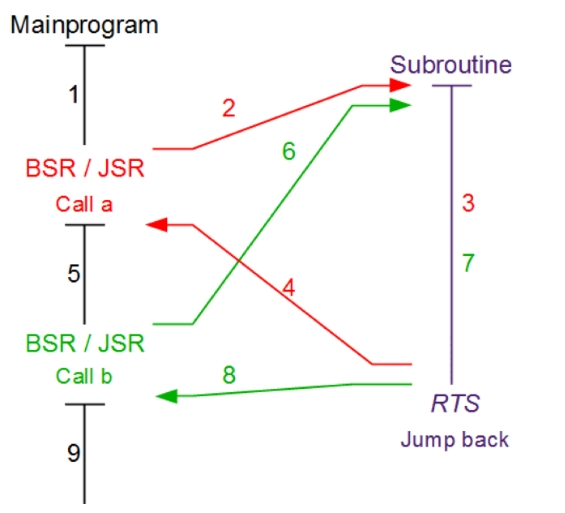
\includegraphics[keepaspectratio=true,height=15\baselineskip]{subroutine.jpg}
	\caption{Process of a subroutine}
	\label{fig:}
\end{wrapfigure}

Per definition, a subroutine is \textit{a sequence of computer instructions for performing a specified task that can be used repeatedly}. So in other words, a subroutine is a \textbf{method}. A subroutine has its own scope, so e.g. variables defined in a subroutine won't be accessible from the main-program. 

The process of a subroutine can be divided into five rough steps:

\begin{enumerate}
	\item Save Program Counter to the Stack
	\item Load the called subroutine
	\item Execute the loaded subroutine
	\item Get the Program Counter from the Stack
	\item Return to Program Counter + 2 \\
	(PC + 1 = \code{BSR/JSR})
\end{enumerate}

\newpage

Of course, subroutines have both pros and cons, however, there are far more pros than cons:
\begin{multicols}{2}
	\paragraph{Pros} \mbox{}\\
	\begin{itemize}
		\item Repeaded command sequences are stored only once in memory \\
			$\rightarrow$ Less memory usage
		\item Repeated command sequences are programmed and tested only once \\
			$\rightarrow$ Less development effort
		\item Programs can be built in a modular way \\
			$\rightarrow$ Lower risk of errors
		\item Programs can be developed by multiple persons at the same time \\
			$\rightarrow$ Higher productivity
		\item Parts of the program can be compiled independent of each other \\
			$\rightarrow$ Shorter compile time, libraries with standard functions
	\end{itemize}
\columnbreak
	\paragraph{Cons}\mbox{}\\
	\begin{itemize}
		\item The call of the subroutine, parameter passing and the return jump need additional time and resources\\
			$\rightarrow$ Slower program execution
	\end{itemize}
		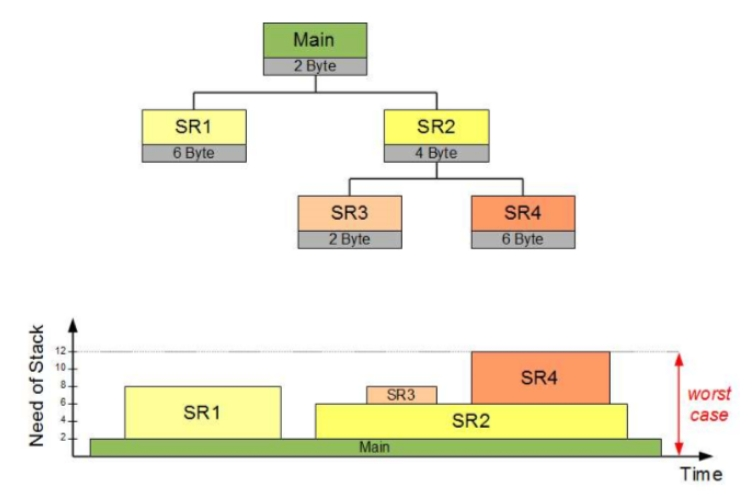
\includegraphics[keepaspectratio=true,height=13\baselineskip]{stack_consumption.jpg}
		\captionof{figure}{Stack consumption on subroutines}
		\label{fig:stack_consumption}
\end{multicols}

\section{Interrupts}
Interrupts are a MCs way of handling exceptions. An Interrupt can react automatically to events and interrupt the main-program to execute a subroutine. However, the state of the main-program has to be preserved, so that after the execution of the subroutine, the main-program can continue at the point where it was before the interrupt. 

\vspace{10px}

\noindent Another, less efficient method of exception handling would be \textbf{polling}, where a service keeps asking the main-program if a certain thing has already happened yet. If it did, the subroutine is executed, if it hasn't, the service will keep asking. That way, the time of the interrupt can be easily foreseen, but it takes a lot more resources to make a request every $x$ milliseconds compared to just setting an interrupt.

\begin{wrapfigure}[13]{R}{0.55\textwidth}
	\centering
	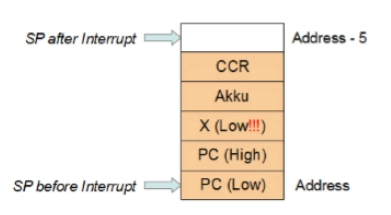
\includegraphics[keepaspectratio=true,height=10\baselineskip]{save_interrupt.jpg}
	\caption{Automatic save of the CPU-state}
	\label{fig:saveInterrupt}
\end{wrapfigure}

\vspace{10px}

\noindent As mentioned before, the state of the main-program needs to be saved before jumping into a subroutine. In contrast to a manual subroutine call with \code{BSR/JSR}, the CPU-state will be saved to the stack \textbf{automatically} (fig. \ref{fig:saveInterrupt}). However, the H-register must be saved manually, if it should be preserved.

\vspace{10px}

\noindent The CPU also needs a so-called \textbf{interrupt-vector}, which sits at a predefined address in the memory. Once an interrupt is triggered, the CPU jumps to the corresponding vector, which points at the start-address of the interrupt-subroutine, so the CPU knows where the subroutine starts.
\vspace{10px}

\noindent By default, the MC doesn't support nested interrupts. So if the program is already in an interrupt-subroutine, it will not go into a second, 'deeper' subroutine, but will queue the second subroutine. Different interrupts have different priorities. The interrupt with the \textit{lowest interrupt-vector number} has the \textit{highest priority} and will therefore be executed first thing after the current subroutine is done.

\begin{figure}[htb]
	\centering
	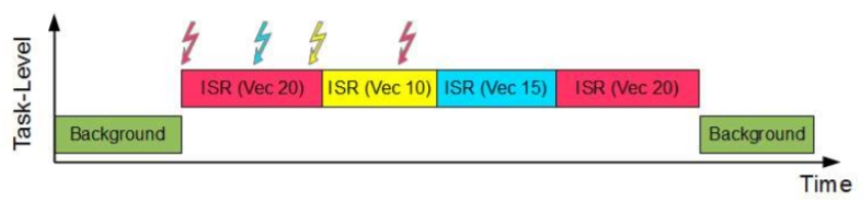
\includegraphics[keepaspectratio=true,height=7\baselineskip]{interrupt_priority.jpg}
	\caption{Queued interrupt subroutines with different priorities}
	\label{fig:interrupt_prio}
\end{figure}

\paragraph{Programming Interrupts}\mbox{}\\
While programming interrupts,some things have to be kept in mind:

\begin{itemize}
	\item Interrupts rely on a \textbf{Stack} to preserve the main-program state
	\item Interruptvectors have to be defined with the start-address of the ISR
	\item Once an interrupt is triggered/fired, its interrupt-flag has to be deleted, because else the interrupt would fire right again, causing an infinite interrupt-loop
	\item Save the H-Register before jumping to an ISR (if needed)
	\item Delete the interrupt flag in the ISR after execution, because else the interrupt will only fire exactly once
	\item Use \code{CLI} to release the interrupts globally
\end{itemize}

\section{Timer}
\begin{figure}[htb]
	\centering
	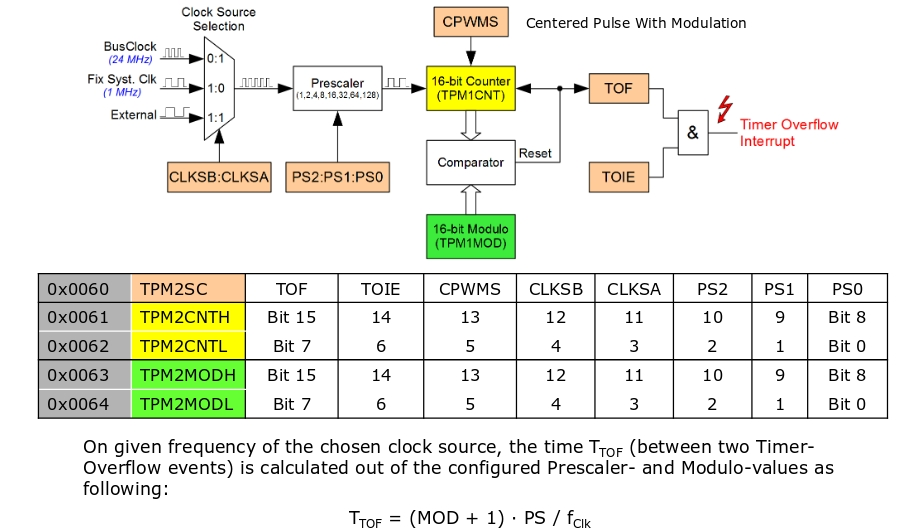
\includegraphics[keepaspectratio=true,height=15\baselineskip]{timer.jpg}
	\caption{Overview of the timer-system in the MC}
	\label{fig:timer}
\end{figure}


In the top-right corner of fig. \ref{fig:timer} a multiplexer can be seen. There, you can select from which clocks the ticks should be counted from:
\begin{multicols}{2}
	\begin{description}
		\item[\code{0:0}] Clock is off
		\item[\code{0:1}] Bus-Clock (24MHz in our case)
		\item[\code{1:0}] Fix System Clock (Set to 1MHz)
		\item[\code{1:1}] External Clock
	\end{description}
\end{multicols}

Afterwards, the clock-signal pass through the \textbf{prescaler}. If you were to set a timer that counts every tick of a 24MHz clock, you would need to set the timer ridiculously high or it would be done within microseconds.

The prescaler can be set to 1, 2, 4, 8, 16, 32, 64 or 128 and filters the ticks. If you were to set the prescaler to e.g. 16, then it would only let every 16-th tick pass. 

Every tick that passes the prescaler increases the 16-bit counter by one. This counter compares its new value with the value of the comparator, which itself gets its value from the 16-bit Modulo, which is set by the user. As soon as the values of the counter and the comparator match, it triggers a reset that resets the counter to 0 and triggers a TOF, a Time Overflow Flag. If the TOIE, the Time Overflow Interrup Enabler is enabled, the TOF triggers an interrupt, that can e.g. start a subroutine.

\vspace{10px}

\noindent The time (in seconds) to trigger the TOF can be calculated with the formula

\[ \scalebox{1.5}{$T_{TOF} = (Modulo + 1) * PrescalerValue * ClockFrequency $} \]

\noindent The Modulo, in turn can be calculated easily if you know the time in seconds, the Prescaler-Value and the clock frequency:

\paragraph{Example}\mbox{}\\
The desired Time $T_{TOF}$ is 3300ms, so 3.3 sec \\
The Prescaler is set to 128, as 3.3sec is quite a lot of time \\
We take the 1MHz ( = 1'000'000Hz) Clock, as 3.3sec is quite a lot of time

$
Modulo = \dfrac{T_{TOF}}{(\dfrac{PrescalerValue}{ClockFrequency})} - 1 = \dfrac{3.3}{(\dfrac{128}{1'000'000})} - 1 = 25780.25 = 25780
$

This timer would be initialized with the following code: 
\begin{lstlisting}[caption={Timer initialization}]
interrupt void myTofISR(void){
	//Method is registered in the .prm Linker-File
	
	//First of all, the Interrupt-Overflow flag has to be reset
	TPM1SC_TOF = 0;
	
	//Do whatever you want to do in this Interrupt-Subroutine
}

void initTimer(void){
	//Set the modulo to the calculated 25780 (or in HEX 64B4)
	TPM1MODH = 0x64;	//Modulo High of Timer 1
	TPM1MODL = 0xB4;	//Modulo Low of Timer 1
	
	//Alternatively, just put TPM1MOD = 25780;
	
	//Set Clock to 1MHZ (See timer-figure)
	TPM1SC_CLKSA = 0;
	TPM1SC_CLKSB = 1;
	
	//Set Prescaler to 128 (128 is the 8.th lowest value --> 111)
	TPM1SC_PS0 = 1;
	TPM1SC_PS1 = 1;
	TPM1SC_PS2 = 1;
	
	//Enable the TOF-Interrupt
	TPM1SC_TOIE = 1;
	
	//reset TOF-Interrupt Flag
	TPM1SC_TOF = 0;
}

void main(){
	initTimer();
	
	EnableInterrupts;
}
\end{lstlisting}

Additional to a single timer, you can also add \textbf{Channels}. Timer 1 has 6 channels (0-5) while Timer 2 has 2 channels (0-1) \\
The Channel-Value (the value, where the channel-interrupt will be triggered) can be calculated with the formula:

\[ \scalebox{1.5}{$Channel Value = \dfrac{T_{ChnF}}{(\dfrac{1}{(\dfrac{ClockFreqency}{PrescalerValue})})}$} \]

\paragraph{Example}\mbox{}\\
Additional to the 3.3 seconds of the timer, another channel-interrupt should fire every second.

The channel value for Channel 0 on Timer 1 ($T_{Ch0F}$)is \\

\begin{center}
$
Channel Value = \dfrac{1}{(\dfrac{1}{(\dfrac{1'000'000}{128})})} = 7812.5 = 7812
$
\end{center}
\newpage

\begin{lstlisting}
interrupt void myCH0FISR(void){
	//ISR is again registered in the linker file
	
	//reset channel interrupt flag
	TPM1C0SC_CH0F = 0;
	
	//Set new Channel Value, so it will fire again after a second
	TPM1C0V = 7812;
	
	//Do stuff
}

void initChannel(void){
	//Set Channel 0 into Output Compare mode
	TPM1C0SC_MS0A = 1;
	TPM1C0SC_MB0B = 0;
	
	//Set Channel 0 into Toggle output on compare
	TPM1C0SC_ELS0A = 1;
	TPM1C0SC_ELS0B = 0;
	
	//Set Channel value to Counter-Value + 7812
	TPM1C0V = TPM1CNT + 7812;
	
	//Enable and reset Channel 0 interrupt
	TPM1C0SC_CH0IE = 1;
	TPM1C0SC_CH0F = 0;
}

void main(void){
	initTimer();
	
	initChannel();
	
	EnableInterrupts;
}
\end{lstlisting}

\noindent Channels can be set into \textbf{input compare} or \textbf{output compare} mode:

\begin{description}
	\item[Input Compare: ] Can only be used with fixed pins. Each time when a signal is being sent through the assigned pin, the value of the timer-counter is written into the channel-value. This can be useful for e.g. stopping time with an external signal.
	\item[Output Compare: ] Compares a fixed value (channel value) with the timer-counter and fires an interrupt each time they match. The channel value can be changed at any time to generate different frequencies. \\
	The Channel value has to be set anew after every interrupt. This can be the same channel value as last time for an even frequency or a different one for a different frequency.
\end{description}

\newpage

\section{PWM}
PWM stands for Pulse Width Modulation and can be used to quickly toggle a signal e.g. to dim an LED. It basically just means that the timer-counter is incredibly low so the interrupt to turn the LED on and off is fired like 30 times per second. The human eye then perceives the LED as dimmed, as it can't see the individual turning on/offs of the LED.

\vspace{10px}

\noindent The PWM can be set to either High-True or Low-True pulses:

\begin{description}
	\item[High-True: ] true = 1. As long as the channel value $>$ timer-counter, the pin is on 1
	\item[Low-True: ] true = 0. As long as the channel value $>$ timer-counter, the pin is on 0
\end{description}

There's also a difference between \textbf{Edge-aligned} and \textbf{Center-aligned} PWM. Center-Aligned PWMs count up to the timer-counter and then count down to 0 again, whereas Edge-Aligned PWMs count up to the timer-counter and then drop directly to 0 to start counting again.

\paragraph{Example}\mbox{}\\
The Front Blue LED is to be dimmed to 30\% with PWM. This LED is coupled to Channel 2 of timer 1 (TPM1CH2). We will use the bus-clock (24MHz) and the timer-counter is insanely low with $2^{16}-1$

\begin{lstlisting}
void initTimer(void){
	//Set Clock to Busclock
	TPM1SC_CLKSA = 1;
	TPM1SC_CLKSB = 0;
	
	//Set Prescaler to 0
	TPM1SC_PS0 = 0;
	TPM1SC_PS1 = 0;
	TPM1SC_PS2 = 0;
	
	//Set timer-counter
	TPM1MOD = 65534
}

void initPWM(void){
	//Set Channel 2 to Edge-Aligned mode
	TPM1C2SC_MS2A = 1;
	TPM1C2SC_MS2B = 1;
	
	//Set Channel 2 to Low-True pulse (LED shines on 0)
	TPM1C2SC_ELS2A = 1
	TPM1C2SC_ELS2B = 1
	
	//Set Channel 2 value to timer-counter * 0.3, so the LED shines with 30% intensity
	TPM1C2V = TPM1MOD * 0.3;
}

void main(){
	PTFDD_PTFDD0 = 1 //Turn off LED
	initTimer();
	initPWM();
	for(;;);	//Neverending loop to not leave main
}
\end{lstlisting}

\end{document}
